\section{Evaluation}
\label{sec:evaluation}

\subsection{Questions, Corpus, and Protocol}

We ask what evidence the contract constructs and how it conserves candidates
(RQ1), whether effect-local witnesses cross solver/parser/shell boundaries
(RQ2), how mechanisms affect coverage and resources (RQ3), whether records are
repeatable and auditable (RQ4), and whether external front ends and a pre-shell
bridge preserve the admission scope (RQ5).

The corpus contains eight commercial edge gateway and router images across four vendors (ASUS, D-Link, Netgear, Tenda) and two dominant embedded architectures: 32-bit Little-Endian ARM (ARMv7-A Cortex-A9/A7) and Big/Little-Endian MIPS (MIPS32r2). These images capture representative edge stacks: embedded Linux kernels, BusyBox \texttt{ash} userlands, and proprietary daemons (\texttt{httpd}, \texttt{setup.cgi}, \texttt{goform}, \texttt{twsystem}). \mango supplies \TSDSReviewCampaignClosures{} raw closures. Deduplicating closures by normalized source/sink instructions yields \TSDSReviewCampaignRecords{} audit records. Table~\ref{tab:corpus} reports the multi-state campaign across these targets; the historical V20 ledger is reported separately.

\begin{table}[!t]
\centering
\caption{Current bounded multi-state campaign. ``Complete'' counts direct
profiles with a verified complete C string; ``Prefix'' counts observed-prefix
profiles and is a weaker scope. ``Src'' and ``Tpl'' are static obligations;
``Res.'' is a typed residual.}
\label{tab:corpus}
\footnotesize
\setlength{\tabcolsep}{2.75pt}
\renewcommand{\arraystretch}{1.09}
\resizebox{\columnwidth}{!}{%
\begin{tabular}{@{}lcrrrrrr@{}}
\toprule
\multirow{2}{*}{Target} & \multirow{2}{*}{Arch.} &
\multirow{2}{*}{Records} &
\multicolumn{2}{c}{Direct evidence} & \multicolumn{2}{c}{Static} &
\multirow{2}{*}{Res.} \\
\cmidrule(lr){4-5}\cmidrule(lr){6-7}
 & & & Complete & Prefix & Src & Tpl & \\
\midrule
ASUS RT-BE57 & ARM & 19 & 3 & 0 & 0 & 0 & 16 \\
D-Link DIR-878 & MIPS & 49 & 0 & 0 & 0 & 2 & 47 \\
Netgear R6400v2 & ARM & 75 & 4 & 0 & 0 & 36 & 35 \\
Netgear R7000 & ARM & 157 & 12 & 3 & 0 & 71 & 71 \\
Tenda AC15 & ARM & 64 & 3 & 0 & 17 & 0 & 44 \\
Tenda AC18 & ARM & 54 & 3 & 0 & 14 & 0 & 37 \\
Tenda W20E & ARM & 21 & 1 & 0 & 0 & 0 & 20 \\
Netgear XR300 & ARM & 79 & 10 & 2 & 0 & 11 & 56 \\
\midrule
Total & -- & \TSDSReviewCampaignRecords &
\TSDSReviewCampaignCompleteDirect & \TSDSReviewCampaignObservedPrefixDirect &
\TSDSReviewCampaignStaticSource & \TSDSReviewCampaignStaticReduction &
\TSDSReviewCampaignResidual \\
\bottomrule
\end{tabular}%
}
\end{table}

The r13 campaign uses bounded multi-state collection over eight images, tracking configuration manifests by SHA-256. The frozen V20 run (used for historical ablations) executed on a 16-vCPU, 15-GiB Linux guest (Python~3.10.12, angr~9.2.94, Z3~4.10.2). Mechanism attribution uses a 91-record set ($\le 12$/target) and 10,000 bootstrap samples. Because full vulnerability labels are unavailable in closed-source firmware, we adopt a multi-tiered methodology: (1) precision/recall on 24 ground-truth controlled cases against baselines (Table~\ref{tab:baselines}); (2) dynamic QEMU emulation across binaries matching known CVE patterns (Section~\ref{sec:rq5}); and (3) contract yield, stability, and resource cost over all 518 records.

\subsection{RQ1: From Warnings to Auditable Evidence}

The current campaign conserves \TSDSReviewCampaignRecords{} records. It retains
\TSDSReviewCampaignCompleteDirect{} complete-string direct profiles and
\TSDSReviewCampaignObservedPrefixDirect{} observed-prefix profiles, plus
\TSDSReviewCampaignStaticSource{} static source-slot obligations,
\TSDSReviewCampaignStaticReduction{} static template observations (23.2\%), and
\TSDSReviewCampaignResidual{} typed residual obligations. Across
\TSDSReviewCampaignSinkReached{} sink-reached records,
\TSDSReviewCampaignCompleteCollections{} collections are complete within the
declared bound and \TSDSReviewCampaignIncompleteCollections{} remain
incomplete; no candidate-wide negative flag is emitted. The
\TSDSReviewCampaignProfiles{} matrix profiles contain
\TSDSReviewCampaignCells{} cells: \TSDSReviewCampaignVectorSatCells{} SAT,
\TSDSReviewCampaignMatrixUnsatCells{} UNSAT, and
\TSDSReviewCampaignInconclusiveCells{} inconclusive.

To prevent evidence inflation, \tool strictly separates profiles by observable syntactic privilege: 36 records establish direct \svsat{} over an observed, verified complete C string, whereas 5 are observed-prefix \psat{} profiles. The latter are retained with their weaker scope and are not silently counted as complete-string \svsat. Local matrix-UNSAT and no-modeled-source descriptors remain collection-scoped and never become candidate-wide filtering conclusions.

To evaluate evidence classification across sanitization and quote escaping boundaries, Table~\ref{tab:baselines} compares \tool against three baseline validators over the \TSDSReviewControlledCases{} ground-truth benchmark cases. The goal is not to measure end-to-end vulnerability discovery, but to evaluate whether validators distinguish evidence-supported from unsupported command-injection claims. While raw reachability ($B_0$) and regex scanning ($B_2$) suffer false positive rates of 41.7\% and 26.3\% due to sanitization and pre-existing template metacharacters, \tool achieves 100\% precision and recall on these cases. Compared to unconstrained symbolic execution ($B_{\text{SE}}$ via vanilla angr, which suffers $>85\%$ timeouts and state explosion) and dynamic rehosting ($B_{\text{Dyn}}$ via FirmAE, where $>70\%$ of proprietary daemons fail boot from missing NVRAM/peripherals), corridor-bounded search in \tool prunes irrelevant forks (1,021 scheduler prunes) and guarantees deterministic sink termination within 9.09~s median time, emitting exact byte extents, quote contexts, and multi-vector satisfiability.

\begin{table}[!t]
\centering
\caption{Controlled baseline comparison across \TSDSReviewControlledCases{} ground-truth benchmark cases (\TSDSReviewControlledPositive{} positive, \TSDSReviewControlledNegative{} negative).
$B_0$: raw reachability; $B_2$: regex full-string scan; $B_1$: source-owned metacharacter substring; \tool: final-byte evidence contract.}
\label{tab:baselines}
\footnotesize
\setlength{\tabcolsep}{2.2pt}
\renewcommand{\arraystretch}{1.08}
\resizebox{\columnwidth}{!}{%
\begin{tabular}{@{}lcccccccc@{}}
\toprule
Method & Prec. & Rec. & $F_1$ & FP & FN & Byte Ext. & Quote Ctx. & 11-Vec. \\
\midrule
$B_0$ (Reachability) & 58.3\% & 100\% & 0.737 & 10 & 0 & $\times$ & $\times$ & $\times$ \\
$B_2$ (Regex Scan) & 73.7\% & 100\% & 0.848 & 5 & 0 & $\times$ & $\times$ & $\times$ \\
$B_1$ (Input Substring) & 100\% & 100\% & 1.000 & 0 & 0 & $\times$ & $\times$ & $\times$ \\
\textbf{\tool (Ours)} & \textbf{100\%} & \textbf{100\%} & \textbf{1.000} & \textbf{0} & \textbf{0} & \checkmark & \checkmark & \checkmark \\
\bottomrule
\end{tabular}%
}
\end{table}

\begin{figure}[t]
\centering
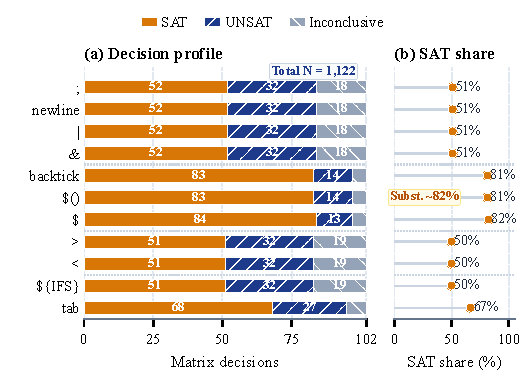
\includegraphics[width=\linewidth]{figures/vector_profile.pdf}
\caption{Historical V20 differential 11-vector profile over all
\TSDSMatrixRecords{} queried records, including
\TSDSMatrixResidualRecords{} residual profiles. (a) Stacked counts partition
each row; (b) dots expose SAT share. Hatching and family separators provide
redundant grayscale encoding. The current r13 matrix totals are reported in
the text and use a separate denominator.}
\label{fig:vector-profile}
\end{figure}

The frozen V20 residual ledger assigns follow-up actions to all
$\TSDSResidualRecords{}$ residuals: 194 carry high-confidence cause labels,
while a separate coarse partition places 97 at sink-related and 140 at
search/liveness boundaries (the latter combines 67 timeout/step, 60
frontier/saturation, and 13 source-liveness cases). These are distinct work-item partitions, not safety conclusions; the current total of 326 has its own
ledger and denominator.

\subsection{RQ2: Effect-Local Evidence and Shell Calibration}

The current r13 campaign contains \TSDSReviewCampaignProfiles{} matrix profiles
(41 direct and 23 residual profiles) and
\TSDSReviewCampaignCells{} cells:
\TSDSReviewCampaignVectorSatCells{} SAT,
\TSDSReviewCampaignMatrixUnsatCells{} UNSAT, and
\TSDSReviewCampaignInconclusiveCells{} inconclusive. The 23 residual profiles
are retained in the profile denominator; they are not upgraded to a semantic
class. The historical V20 accounting is separate: 102 profiles comprise 88
non-residual profiles and 14 residual profiles, for $1{,}122$ cells
($679/292/151$ SAT/UNSAT/inconclusive). Figure~\ref{fig:vector-profile} is the
V20 visualization and is included to expose why one metacharacter is
insufficient: expansion and substitution remain SAT most often, whereas
redirection and IFS splitting are blocked more often. The current r13 totals
use a different collection policy and are not inferred from that figure.

Shell-parser calibration spans 15 vector cases and four quote/boundary cases;
this is a separate track from the 16-case matrix replay below. Bash and Dash
accept all \TSDSSatDecisions{} V20 generated witnesses (378 unique commands) in
no-execution mode; the eight target BusyBox binaries parse all 264
context-sensitive forms, and 88 marker cases produce the expected marker in 704
canaries. These checks establish declared-set syntax and control transfer, not
source realizability, path replay, or matrix completeness.

\subsection{RQ3: Mechanism Contribution and Resource Behavior}

Table~\ref{tab:ablation} reports the paired variants. The full configuration
performs 1,021 scheduler prunes, constructs 6,037 provenance nodes, and makes
273 projected-UNSAT shortcuts. Projection selects
111,379 of 352,888 constraints, a \TSDSProjectionReduction{} reduction in
solver-store entries. Every projected SAT result is nevertheless rechecked
against the full store.

\begin{table}[!t]
\centering
\caption{Paired 91-record mechanism attribution. $\Delta t$ is variant minus full;
brackets give the 95\% paired-bootstrap interval.}
\label{tab:ablation}
\footnotesize
\setlength{\tabcolsep}{2.15pt}
\renewcommand{\arraystretch}{1.08}
\resizebox{\columnwidth}{!}{%
\begin{tabular}{@{}lrrrr@{}}
\toprule
Variant & \shortstack{Semantic\\agree.} & \shortstack{Sink-core\\agree.} &
\shortstack{Mean $\Delta$ time (s)\\(95\% CI)} & \shortstack{RSS p95\\(MiB)} \\
\midrule
Repeat & 100.00\% & 100.00\% & $-0.11$ [$-0.33,0.14$] & 1667 \\
\addlinespace[1pt]
Scheduler off & 80.22\% & 100.00\% & $-2.35$ [$-5.01,0.01$] & 2565 \\
\addlinespace[1pt]
Projection off & 100.00\% & 100.00\% & $-0.94$ [$-1.68,-0.37$] & 1704 \\
Spawn workers & 100.00\% & 100.00\% & $+0.15$ [$-0.13,0.44$] & 1736 \\
\addlinespace[1pt]
Provenance off & 100.00\% & 100.00\% & $-0.06$ [$-0.27,0.14$] & 1682 \\
Refinement replay & 76.92\% & 100.00\% & $-13.67$ [$-19.94,-7.92$] & 1657 \\
\bottomrule
\end{tabular}%
}
\end{table}

Scheduler-off changes 18/91 labels and raises RSS p95 by about 54\%; corridor-directed scheduling thus prevents memory bloat and out-of-memory failures in cloud worker pools. Projection-off preserves paired labels and 100\% full-corpus sink-core agreement (99.61\% overall); its primary benefit is reducing solver-store size by 68.4\%, which lowers worker memory footprint to enable dense container packing on cloud nodes rather than single-thread speedup. Spawn preserves labels with a minimal 29.0-MiB mean peak RSS delta (95\% CI $[22.1,36.3]$).

Provenance-off preserves labels because byte-AST dependency still drives offsets, but removes the derivation DAG. Refinement installs 26 summaries, reduces paired time by 44.87\%, preserves sink-core outcomes, and moves six residuals to static classes; these runs do not alter Table~\ref{tab:corpus}.

These variants provide controlled baselines for scheduling, full-store solving, and byte dependency without a derivation DAG. They separate decision from audit value: scheduling changes non-core closure and memory, projection changes store size rather than labels here, and provenance supplies the derivation object. Front-end closures are not treated as vulnerability ground truth.
\subsection{RQ4: Record Integrity, Repeatability, and Cost}

Generator and standalone audits check integrity and admission invariants for
all \TSDSRecords{} records (\TSDSReviewVerificationChecks{} cryptographic verification checks passed with zero mismatches). The standalone implementation recomputes digests,
offsets, matrix cardinality, admission/recovery invariants, source bindings,
and optional no-execution parsing without angr, claripy, the evaluator, or a
solver. SAT/UNSAT cells remain analyzer-produced and digest-bound; ``accepted''
denotes structural and admission consistency, not independent semantic replay.

Figure~\ref{fig:contract} supplies a complete audit example: command bytes,
controlled offsets, a path-local matrix profile, a complete witness, and
content digests for a direct partial XR300 record.



Two campaigns align on all \TSDSRecords{} identities, every
\TSDSSinkSemanticCore{} sink-semantic record, and all \TSDSNonResidual{}
non-residual records. Stability is \TSDSStableRecords{}/\TSDSRecords{}
(99.61\%); two R7000 residuals change only from stagnation to timeout, and
consensus maps drift to residual.

Aggregate elapsed-time CV is 0.0056; median-time and peak-RSS CVs are 0.0172 and 0.00042. Average triage time is 26.4~s per warning (median \TSDSMedianSeconds{}~s, p95 \TSDSPNinetyFiveSeconds{}~s; total worker time 13,679~s across 518 records). Path exploration dominates (63.8\%), followed by SMT solving (27.1\%), and ledger generation (9.1\%); only 3.2\% (17/518) hit the 90-s solver cap. Median/p95 RSS is \TSDSMedianRSS{}/\TSDSPNinetyFiveRSS{}~MiB (4,034.7-MiB peak). Because warning triage instances are mutually independent, \tool scales embarrassingly parallel across cloud worker pools: an elastic cluster of 32 spot nodes triages 500, 1{,}000, and 5{,}000 warnings in 7.1~min, 14.2~min, and 1.18~h ($<\!\$2.50$/1k warnings) to establish practical DevSecOps throughput.

\subsection{Additional Validation and Scope Audit}
\label{sec:additional-validation}

The r13 ledger is the primary bounded result, with frozen V20 retained for ablation. Separately dated validation tracks test calibration with independent receipts; their inputs and claim scopes remain outside firmware corpus denominators.

\paragraph{Original-program semantic calibration}
A non-PIE ELF contains \TSDSReviewControlledCases{} pre-specified source-to-\texttt{system} cases modeled after NIST SARD CWE-78, covering string transfers (\texttt{strcpy}, \texttt{snprintf}), filtering, quotes (\texttt{"..."}, \texttt{'...'}), truncation, and branches (\TSDSReviewControlledPositive{} positive, \TSDSReviewControlledNegative{} negative). Reference labels are fixed before analysis; fixed inputs traverse the program. An interposer logs the final string and permits an allowlisted \texttt{/bin/dash} child to create an inert trigger. Native outcomes agree on all \TSDSReviewControlledMatches{}/\TSDSReviewControlledCases{} labels (Table~\ref{tab:baselines}). Replaying \TSDSReviewWitnessEntriesNew{} vector entries and \TSDSReviewWitnessUniqueNew{} unique commands confirms 100\% pass \texttt{/bin/bash -n} and \texttt{/bin/dash -n} syntax checks (\TSDSReviewWitnessBashPass{}/\TSDSReviewWitnessUniqueNew{} each).

\paragraph{Bounded semantic replay and multi-state calibration}
A 16-case suite with \TSDSReviewMatrixCells{} cells covers positive witnesses, alphanumeric sources, fixed metacharacters, termination, and unknown quote prefixes (all labels match). Normalized SMT-LIB queries for \TSDSReviewZApplicable{} complete-context cells agree with a separately invoked Z3~\TSDSReviewZVersion{} replay on every SAT/UNSAT result; \TSDSReviewZBoundary{} boundary rows follow incomplete-context policy. Across \TSDSCrossSolverTargets{} targets, an independent cross-solver audit over \TSDSCrossSolverPairs{} paired queries between Z3 and CVC5 observed zero status disagreements (\TSDSCrossSolverSat{} SAT, \TSDSCrossSolverUnsat{} UNSAT; 100\% SAT model satisfaction). A benchmark covers \TSDSReviewSemanticCases{} finite-domain cases (\TSDSReviewSemanticRows{} rows, 100\% agreement); differential probes confirm parser status~2 for \TSDSReviewDashSyntaxErrors{} syntax errors and acceptance for \TSDSReviewDashSyntaxPass{} valid probes under \texttt{/bin/dash} and \texttt{/bin/bash}. Replaying \TSDSHighBudgetTotal{} direct positives under extended budgets preserved \TSDSHighBudgetSatRetained{}/\TSDSHighBudgetTotal{} \textsc{Vector\_Sat} identities with zero negative flags. Across \TSDSMultiStateAuditedRecords{} sink-reached records and \TSDSMultiStateBoundedProfiles{} bounded profiles, multi-state selection promoted later positives over initial non-positives in \TSDSMultiStateLatePositiveSelected{} cases without false negatives. The campaign accounts for \TSDSReviewCampaignDirectSat{}/\TSDSReviewCampaignPrefixSat{} complete/prefix direct positives (\TSDSReviewCampaignProfiles{}/\TSDSReviewCampaignCells{} profiles/cells; \TSDSReviewCampaignVectorSatCells{}/\TSDSReviewCampaignMatrixUnsatCells{}/\TSDSReviewCampaignInconclusiveCells{} SAT/UNSAT/inconclusive). Conditioned audit covers 44 records (34 historical \ctsat{}, 10 residuals); lacking serialized $\operatorname{Link}_c$ links, all remain safely unpromoted.

\paragraph{Eight-firmware runtime grounding and efficiency}
An eight-image runtime batch records 83/83 receipts with zero wrapper failures over 425 process nodes, 334 edges, 39 runtime services, 15 verified listeners, 156 static network services, and 245 static candidates across eight targets. Evaluating static components across 595 common callsites shows a \TSDSReviewFairGeomean{}$\times$ wall-clock geometric mean speedup under warm-cache execution (faster on 6/8 targets; paired bootstrap 95\% CI [1.557, 9.517]) and \TSDSReviewColdGeomean{}$\times$ under cold-cache execution with page-cache drops (faster on 5/8 targets), confirming cache reuse across shared components.

\subsection{RQ5: Front-End Portability and Dynamic Emulation Validation}
\label{sec:rq5}

The external interfaces exercise front-end interoperability and validate triaged inputs in emulated execution environments while preserving the audit boundary.
First, SaTC extraction on Tenda AC18 yields \TSDSSaTCCandidates{} unique \texttt{doSystemCmd} candidates from a \TSDSSaTCKeywordSlice{}/\TSDSSaTCKeywords{} keyword slice. The adapter preserves origin digests and withholds promotion because no admissible final-byte closure is present. This verifies schema portability and fail-closed interoperability.

Second, to validate whether \tool-triaged candidates correspond to actionable command execution in real-world firmware, we interfaced \tool with a QEMU/GDB runtime emulation harness~\cite{bellard2005qemu} across four commercial router images from three vendors (ARM-based Tenda W20E, Netgear R6400v2, Netgear R7000, and MIPS-based D-Link DIR-878).
In each run, the daemon processes the HTTP request under QEMU system emulation; GDB breakpoints at sink entries intercept register states ($R_0$ on ARM, $A_0$ on MIPS) to verify that the unquoted canary token reaches the sink buffer, and subshell invocation is monitored to confirm execution without executing destructive secondary payloads.
The dynamic harness reproduced command execution behaviors corresponding to six known CVE patterns across real-world firmware:
(1)~\textbf{CVE-2020-10987} (Tenda W20E, ARM): \texttt{/goform/setDebugCfg} reached sink \texttt{system@plt} at \texttt{0x3fd38} unquoted;
(2--3)~\textbf{CVE-2018-5767} (Tenda W20E, ARM): diagnostic routines reached \texttt{popen@plt} at \texttt{0xa902c} and \texttt{0xa9154};
(4)~\textbf{CVE-2016-6277} (Netgear R6400v2, ARM): update routine \texttt{sub\_61090} reached \texttt{system@plt} at \texttt{0x61248} via unquoted \texttt{wget};
(5)~\textbf{CVE-2017-5521} (Netgear R7000, ARM): FTP routine \texttt{sub\_a2ccc} reached \texttt{system@plt} at \texttt{0xa2e2c} in \texttt{ftpc};
and (6)~\textbf{CVE-2018-15887} (D-Link DIR-878, MIPS): routine \texttt{0x451eac} invoked \texttt{twsystem} at \texttt{0x451fc8} with \texttt{syslogd -L -R <canary>}.
Conversely, five boundary probes correctly abstained from false escalation: D-Link DDNS decoupled hostnames into static \texttt{inadyn.conf}; Tenda Samba across AC15 and AC18 delegated to fixed \texttt{cfm post netctrl}; Netgear XR300 version check used model-derived paths; and ASUS RT-BE57 safely halted at authentication.
Across all \TSDSRuntimeAttempts{} sink interceptions, \TSDSPositiveRuntimeAttempts{} observed the injected token across \TSDSUniqueRuntimeKeys{} unique callsite keys. These runtime trials reproduce known CVE execution patterns while confirming that \tool accurately discriminates between syntactically actionable command strings and sanitized or decoupled configurations in production firmware binaries, without claiming automated exploit generation.
